\section{氧气的制取和性质}\label{sec:xssy-sy3}

\begin{shiyanmudi}
    1. 学会实验室制氧气的方法,并试验氧气的性质; 2. 学会用排水法收集气体。
\end{shiyanmudi}


\begin{shiyanyongpin}
    大试管、试管夹、单孔橡皮塞、橡皮管、导管、集气瓶(125 毫升)、水槽、铁架台(带铁夹)、坩埚钳、酒精灯、玻璃片、燃烧匙、木条。

    氯酸钾、二氧化锰、高锰酸钾、木炭、红磷、棉花、石灰水。
\end{shiyanyongpin}

\begin{shiyanbuzhou}
    1. 二氧化锰对氯酸钾分解的催化作用

    观察氯酸钾和二氧化锰的颜色、状态。

    在一洁净\footnote{做这个实验,试管必须洁净,特别是管壁上不能附着有机物杂质,否则容易发生爆炸,造成事故。}
    而干燥的试管里加入约 $0.5$ 克氯酸钾,用试管夹夹住试管进行加热,使氯酸钾熔化。取带火星的木条伸入试管。
    观察发生的现象。这时候有没有氧气放出?把试管撤离火焰,撒入少量二氧化锰粉末,立即把准备好的带火星的木条伸入管内。
    观察到什么现象?从这个实验得出什么结论?

    2. 用加热分解高锰酸钾的方法制取氧气

    观察高锰酸钾的颜色和状态。

    用带有导管的橡皮塞塞紧试管。检查这个装置是否漏气。
    拔开橡皮塞,在上述试管里放进大约 7 克的高锰酸钾。
    用一团棉花放在靠近试管口的地方,以防止加热时高锰酸钾粉末进入导管。
    然后把带有导管的塞子塞紧试管口。

    用铁夹把这个装置固定在铁架台上(图 \ref{fig:xssy-18})。将集气瓶盛满水,并用玻璃片盖住瓶口%
    \footnote{用玻璃片盖瓶口时,可以先盖住一小部分,随后推动玻璃片.直至把瓶口全部盖住。}
    (注意不要让瓶口水面留有气泡)。把盛满水的瓶子连同玻璃片一起倒立在盛水的水槽内。
    观察瓶底有没有气泡。如果有气泡,就要重新操作。

    \begin{figure}[htbp]
        \centering
        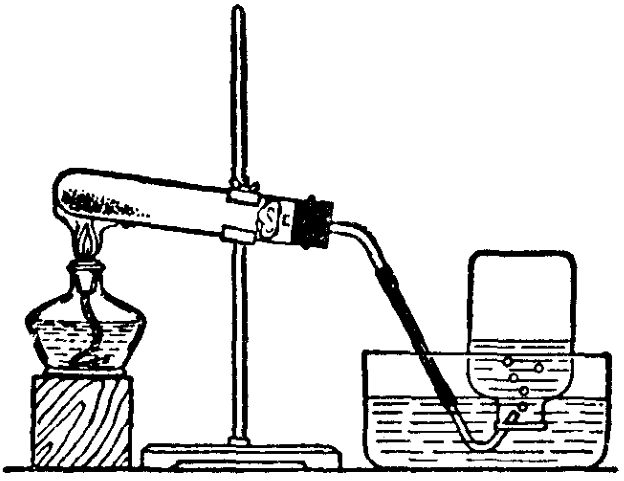
\includegraphics[width=0.5\textwidth]{../pic/czhx1-xssy-18}
        \caption{实验室制取氧气}\label{fig:xssy-18}
    \end{figure}


    给试管加热。先使酒精灯在试管下方来回移动,让试管均匀受热,然后对高锰酸钾所在的部位加热。

    导管口开始有气泡放出时,不宜立即收集,为什么?
    当气泡连续地并比较均匀地放出后,再把导管口伸入盛满水的集气瓶里。
    等瓶子里的水排完以后,(你怎样判断?)用玻璃片盖住瓶口。
    小心地把瓶子移出水槽,正放在桌子上。用同样的方法再收集一瓶氧气。
    停止加热时,先要把导管移出水面,然后熄灭火焰,为什么?

    观察收集到的氧气的颜色,并用带有火星的木条插入集气瓶口检验氧气的存在
    (检验后立即用玻璃片盖住集气瓶口,使瓶里剩余的氧气足够供下面的实验用)。
    记录观察到的现象。

    3. 试验氧气的化学性质

    (1) 木炭在氧气里燃烧 \quad 用坩埚钳夹取一小块木炭在酒精灯的火焰上烧到发红,放在燃烧匙里,立刻插入盛有氧气的集气里。
    观察有什么现象发生。燃烧停止后,取出燃烧匙,往集气瓶里加入少量澄清石灰水,再振荡一下。有什么现象发生?
    木炭在氧气里燃烧,生成什么物质?

    (2) 磷在氧气里燃烧 \quad 取少量红磷放在燃烧匙里,在酒精灯火焰上燃着,注意观察磷在空气里燃烧的情况,
    然后赶快把燃烧匙插入另一盛满氧气的集气瓶里,并立即将玻璃片盖上,观察有什么现象发生。
    比较磷在空气里燃烧和在氧气里燃烧的情况。注意磷燃烧时产生浓厚的白烟,这是五氧化二磷的粉末。
\end{shiyanbuzhou}

\begin{wentihetaolun}

    1. 根据课堂实验和上面的实验,总结氧气的物理性质和化学性质,并填入下表。

    \begin{table}[H]
        \hspace*{4em}\begin{tblr}{
            rowsep=0pt,
            row{1}={abovesep=0.5em, belowsep=0.5em},
            hline{1,8}={1.5pt,solid},
            hline{2}={solid},
            vline{1,5}={1.5pt,solid},
            vline{3}={solid},
            column{2}={6em},
            column{4}={12em},
        }
            \SetCell[c=2]{c}物理性质 & & \SetCell[c=2]{c}化学性质 & \\
            状态(通常情况下)& \xhx[5em] & (1) & 氧气跟非金属反应 \\
            颜色             & \xhx[5em] &     &  \ce{\text{碳} + \text{氧气} ->} \\
            气味             & \xhx[5em] &     &  \ce{\text{硫} + \text{氧气} ->} \\
            密度(跟空气比较)& \xhx[5em] &     &  \ce{\text{磷} + \text{氧气} ->} \\
            溶解性(对水)    & \xhx[5em] & (2) &  氧气跟金属反应 \\
                             &           &    &  \ce{\text{铁} + \text{氧气} ->}
        \end{tblr}
    \end{table}

    2. 收集氧气能不能用向上排空气法?为什么?如果改用向上排空气法收集氧气,实验用品需作什么改动?

    3. 在实验步骤 1、2 中,应根据什么调节试管的高度?

\end{wentihetaolun}

